\documentclass[journal]{./sty/IEEEtran}

\usepackage{graphicx}

% *** CITATION PACKAGES ***
\usepackage{cite}
% cite.sty was written by Donald Arseneau
% V1.6 and later of IEEEtran pre-defines the format of the cite.sty package
% \cite{} output to follow that of IEEE. Loading the cite package will
% result in citation numbers being automatically sorted and properly
% "compressed/ranged". e.g., [1], [9], [2], [7], [5], [6] without using
% cite.sty will become [1], [2], [5]--[7], [9] using cite.sty. cite.sty's
% \cite will automatically add leading space, if needed. Use cite.sty's
% noadjust option (cite.sty V3.8 and later) if you want to turn this off.
% cite.sty is already installed on most LaTeX systems. Be sure and use
% version 4.0 (2003-05-27) and later if using hyperref.sty. cite.sty does
% not currently provide for hyperlinked citations.
% The latest version can be obtained at:
% http://www.ctan.org/tex-archive/macros/latex/contrib/cite/
% The documentation is contained in the cite.sty file itself.


% *** MATH PACKAGES ***
%
\usepackage[cmex10]{amsmath}
% A popular package from the American Mathematical Society that provides
% many useful and powerful commands for dealing with mathematics. If using
% it, be sure to load this package with the cmex10 option to ensure that
% only type 1 fonts will utilized at all point sizes. Without this option,
% it is possible that some math symbols, particularly those within
% footnotes, will be rendered in bitmap form which will result in a
% document that can not be IEEE Xplore compliant!
%
% Also, note that the amsmath package sets \interdisplaylinepenalty to 10000
% thus preventing page breaks from occurring within multiline equations. Use:
% \interdisplaylinepenalty=2500
% after loading amsmath to restore such page breaks as IEEEtran.cls normally
% does. amsmath.sty is already installed on most LaTeX systems. The latest
% version and documentation can be obtained at:
% http://www.ctan.org/tex-archive/macros/latex/required/amslatex/math/


\usepackage{url}


% correct bad hyphenation here
\hyphenation{net-works SpiNNaker depending}

\begin{document}
%
% paper title
% can use linebreaks \\ within to get better formatting as desired
\title{Creating, Removing, and Modifying\\Synaptic Connections On The Spiking Neural Network Architecture (SpiNNaker) In Real-Time
}


\author{Matthew Frazier ~
        Nishant Shukla ~
        Worthy Martin* }

% The paper headers
\markboth{Journal of Neuroscience Methods,~Vol.~x, No.~y, January~2014}%
{Shell \MakeLowercase{\textit{et al.}}: Synaptogenesis on the SpiNNaker}
% The only time the second header will appear is for the odd numbered pages
% after the title page when using the twoside option.


% make the title area
\maketitle

\begin{abstract}
Artificial Neural Networks is a promising approach to study human brain computation in hopes of achieving similar learning by artificial agents.
Recent architecture design of a low-power supercomputer by the University of Manchester (SpiNNaker) has made it easier to design highly parallel brain-inspired algorithms.
We used the SpiNNaker chip to implement a neural network capable of rewiring its connection in real-time while trying to minimize information loss and maximize the decrease in statistical dependence.
Additionally, we explored scalability issues and unintended pitfalls with this approach.

\end{abstract}

\begin{IEEEkeywords}
Neural Networks, Synaptogenesis, SpiNNaker
\end{IEEEkeywords}


\section{Introduction}
\IEEEPARstart{T}{he} subfield of AI known as neural network computation has recently received a large and growing amount of attention. 
Put simply; neural networks (NN) are computational models inspired by biological brains that are capable of machine learning. 
A NN usually consists of interconnected "neurons" (in quotation marks for they are artificially simulated to varying degrees of biological accuracy -- but that topic is outside the scope of this paper) which compute from their inputs and produce various outputs, depending on the model. 

This paper focuses on types of spiking neural network (SNN) models, in which the neuronal communication (and therefore, the computation of the system as a whole) is achieved via message spikes, or action potentials, from one neuron that is synapsed onto another. 
In this introduction, we first describe how a SNN is a good computational representation of the brain. 
We then describe various different spike-dependent spike-time learning methods used on a SNN, followed by an exploration of various types of SNN. 
We discuss why the neuromimetic hardware we use is a good platform for experimentation with SNN, and then describe our approach to the problem of simulating synaptogenesis on such a device and propose a solution. 
Our design section explores this solution in detail, and our implementation section describes our results.
Furthermore, we discuss future work that remains to be conducted, including interesting implications such as computability beyond Von Neuman architecture and Turing machines.

\subsection{The Brain And Other Spiking Neural Networks}
The brain is a spiking neural network. 
That is to say; biological neurons pass information around the brain via action potentials which travel from a neurons' soma (cell body) down the axon and generate synaptic events which are received by the dendrites of all other connected neurons.
Figure 1 diagrams the relevant biological prerequisites.

%\begin{figure}
%\centering
%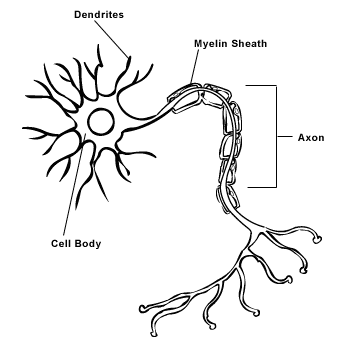
\includegraphics[scale=0.6]{img/neuron}
%\caption{Visual representation of a biological neuron identifying the cell body, dendrites, and axon.}
%\end{figure}


The process has been simplified greatly as neurobiology is not the focus of this paper, nor is the biological process yet completely understood. 
What's important are the overarching properties exhibited by brains. 
Namely; that brains are fast, power-efficient, and capable of obtaining, representing, and integrating complex multi-dimensional information sets into useful knowledge (and from noisy sensory inputs, at that). 
Moreover, the property of being able to fairly reliably solve highly complex problems is something we want computers to have. 
[Include TSP example illustrating that a human could do in a day what a procedural program would take hundreds of thousands of man-years to do?]
Progress is however being made towards the goal of making machines more like minds; indeed, the bus in a computers' hardware may operate at tens of MHz, while an axon may carry only tens to hundreds of action potentials per second, about five orders of magnitude slower than a machine (Furber 2007). 
The power efficiency of the brain is still far ahead of even the best neuromimetic hardware but the gap is closing quickly, considering that biological evolution had several hundred million years of a head start. 

One very important property of the brain that has received little attention by Computer Scientists, which is also believed to be quintessential in mankind's ability to adapt to and solve new and ever-more difficult problems, is neural plasticity involving the dynamic creation or removal of synapses.
It would be erroneous to say that no degree of plasticity has been implemented in any type of SNN, but to the best of our knowledge there is yet no model which allows networks to add or remove synapses at runtime. 
Given that we do not yet fully understand the mechanisms governing neural plasticity in our own heads, it suffices to say that there is yet much work to be done in this field of computational neuroscience in which artificial neural networks dynamically alter their own topology.

\subsection{Overview of Spike-time coding and learning methods}
Before discussing different types of artificial spiking neural networks, it is necessary to describe various spike-time coding and learning methods that are relevant to understanding how the different types of spiking neural networks function.

Firstly, the distinction between rate- and rank-order coding must be addressed. 
Rate order coding is, as it sounds, a way to describe neural responses to stimulus in terms of firing rate, paying attention to the timing between spikes of a single input. 
Rank order, on the other hand, focuses on the relative timing of spikes from all inputs. 
As has been argued in depth elsewhere [cite], rate order has a number of drawbacks, though the primary one is its inability to transmit and process information in a short period of time; with \(n\) neurons being able to transmit over the course of 10 ms only $log_2(n C 1)$ bits of information.
Rank order, under the same constraints, is capable of achieving $log_2(n!)$ bits of information. [cite: Kasabov 2013]

As detailed in [cite: Thorpe 1998], rate order can be considered an $analog-to-frequency$ converter, while rank order would be an $analog-to-delay$ converter, as the time an integrate-and-fire neuron takes to reach threshold is dependent upon input strength. 
During an initial learning phase, in which a new output neuron $i$ is created for each $N$-dimensional training input pattern, connection weights $w_j,i (j = 1,2,...,N)$ are calculated based on the rank order learning rule:

\begin{equation}
w_j,i(t) = {\alpha}\cdot{mod^{order(j,i)}} 
\end{equation} 
where $w_j,i$ is the connection weight between post-synaptic neuron $i$ and pre-synaptic neuron $j$, $\alpha$ is a learning parameter, $mod$ is a modulation factor (determining the importance of the order of the first spikes), with $order(j,i)$ representing the order of spikes arriving at neuron $i$ from all synapses to the neuron $i$ (has value $0$ for the first spike to neuron $i$, increases incrementally for each subsequent spike from other pre-synaptic neurons). [cite: Kasabov 2013]
Some models using rank order coding will also merge output neurons with similar weight vectors based on the Euclidean distance between them, thus reducing the number of redundant neurons that must be simulated.
In short, rank order (RO) coding is assumed to be a better basis for model construction as it allows networks to process more information in a shorter amount of time with fewer redundant neurons. 

Moving on to learning methods, spike time dependent plasticity (STDP) implements plasticity through the use of long-term potentiation (LTP) and depression (LTD). 
In other words, the connection weight between two neurons increases if the pre-synaptic neuron spikes before the post-synaptic neuron, and the weight decreases in the reverse case. 
Spike driven synaptic plasticity (SDSP) is a semi-supervised variant of STDP in which a threshold $Vmth$ is given to the post-synaptic neurons' membrane potential. 
If the membrane potential is above $Vmth$ when an input spike arrives, potentiation occurs. 
Otherwise, the synapse experiences depression.
[edit: use formulas from Kasabov?] 
These two cases are typically either shortly before or shortly after a post-synaptic spike is emitted, respectively. 

We will later describe a new learning method referred to as entropic synaptogenetic plasticity (ESP), governed by biologically inspired formulas taken from (Levy), and influenced by Information Theory from Shannon.

\subsection{Types of Spiking Neural Networks}

\begin{itemize}
\item[(a)] {\bf A spiking neural network (SNN)} is the most basic form, in which synaptic weights are static and neurons communicate via message spikes.
While they have some drawbacks, an SNN is still a fairly powerful biologically-inspired model.
\item[(b)] {\bf An evolving spiking neural network (eSNN)} evolves its functionality and structure based on incoming information using the RO rule -- formula (1), but only during a learning phase.
Once a neurons' weight has been set, however, this model does not allow for any further tuning of synaptic weights to reflect on other incoming spikes at the same synapse. 
That is to say; these synapses can capture some long-term memory during the learning phase, but have little ability to capture any short term memory, which is detrimental to the computational capabilities of the network as a whole. 
\item[(c)] {\bf A dynamically evolving spiking neural network (deSNN)} represents an improvement over eSNN in that it implements not only RO learning during an initial learning phase, but also a dynamic synaptic plasticity mechanism so that it will continue to learn and improve performance during a recall phase; the deSNN proposed in [cite: Kasabov 2013] uses the SDSP mechanism.
This fixes the primary shortcoming of the eSNN model; allowing for short term memory to be stored easily, and to be potentiated as long as it remains useful. 
\end{itemize}

\subsection{SpiNNaker}
The Spiking Neural Network Architecture (SpiNNaker) board is a neuromimetic hardware system designed by the University of Manchester with the eventual intent of simulating the human brain. 
It is the brainchild of Steve Furber, and has a number of properties that make it useful for neural computation:
\begin{itemize}
\item fast
\item power efficient
\item massively parallelized
\item globally asynchronous
\item locally synchronous 
\item capable of running complex SNN simulations [superfluous?]
\item scalable
\end{itemize}
[cite: all of the above]
[TODO: explain why these properties make it suitable for this experiment -- also the overlap of these properties with those of the brain]

\subsection{Synaptic Plasticity}
A difficult problem in designing neural networks is configuring the initial parameters to optimize the network.
For example, defining how the neurons are connected together greatly affects the efficiency and performance in learning [cite]. 
Perceptrons are often designed as bipartite graphs, where every neuron in the pre-synaptic layer is connected to every neuron in the post-synaptic layer.
This brute-force approach to constructing a network topology may achieve satisfactory results if the weights converge to the optimal values within an acceptable time.
However, a bipartite graph scales exponentially to the number of nodes in each layer. 
In our solution, we let the neural network modify itself, providing a ``hands-off'' approach to designing a network.

Other than updating synaptic weights to achieve learning, we introduce two additional forms of synaptic plasticity. 
In our study, we allow new synapses to be formed (synaptogenesis), or existing synapses to be entirely disconnected. 
The three types of plasticity undergo the following principles (Levy 2004):

\begin{itemize}
\item[(a)] {\bf Synaptogenesis} - 
Unlike most networks, we allow ours to form new connections between neurons while learning occurs. 
The creation of a new synapse depends on whether the post-synaptic neuron is at an optimal activation. 
If not, the network considers forming a new synapse.
Additionally, synaptogenesis only occurs between neighboring neurons, ensuring a constraint on locality.
Synapses are formed by taking into account both receptivity and avidity (Levy 2004).

\vspace{0.3cm}

Avidity is the measure of ability for each neuron to participate in a new synaptic connection, defined as

\[
A_i(t)=\frac{a}{(a + \sum_j\sum_kW_{i_kj}(t))}
\]

\[
a = \left\{
\begin{array}{lr}
  1.0 * 10^{33} & \text{for unlimited avidity}\\
  1.0 & \text{for moderate avidity}\\
  1.0 * 10^{-3} & \text{for limiting avidity}
\end{array}
\right.
\]

The receptivity of new synaptic connections is inversely proportional to the running average of the neuron's activation.
We use the following equation for receptivity,

\[
R_j(t) = \frac{r_1}{r_1 + \bar{y}_j(t)^{r_2}}
\]

\[
\bar{y}(t) = 0.99 \bar{y}_j(t-1) + 0.01 Y_j(t)
\]

\[
\text{(\(r_1\) and \(r_2\) are experimental constants)}
\]

Finally, the probability of forming a new synapse between two neurons \(i\) and \(j\) depends on both avidity and receptivity. 

\[
\text{Prob}(\text{of new synapse } ij ) \propto A_i(t) * R_j(t)
\]

\item[(b)] {\bf Weight Modification} - 
Similar to most unsupervised weight modification rules, we use a deterministic process depending on the pre- and post-synaptic activities.
This type of weight adjustment is based off the Hebbian rule, where links between nodes that fire together strengthens.
Specifically, weights are adjusted using the following formula,

\[
\triangle w(t+1) \propto f(\text{post}_j(t))*g(\text{pre}_j(t), w_{ij}(t))
\]

\item[(c)] {\bf Synapse Removal} -
Lastly, we allow our network to undergo synaptic removal, a stochastic process where the probability of removal becomes non-zero if excitatory synapses fall bellow a specified threshold.
Given some constant \(\delta > 0\), probability of synaptic removal is defined as

\[
\text{Prob}(\text{removal } ij) = \left\{
     \begin{array}{lr}
       0 & \text{if } w_{ij}(t) + \triangle w_{ij}(t+1) > \delta\\
       >0 & \text{otherwise}
     \end{array}
   \right.
\]

\end{itemize}

Synaptic connections are slowly modified through additions or removals until optimal output firing levels are obtained. 

Levy asserts that  ``information theory has gained popularity in recent years as a tool for understanding brain recordings.''

\hfill

[TODO: Matt] We're combining the two and extending the deSNN model into an edeSNN model, which will shortly achieve sentience and enslave the entire human race.


\section{Design}
\IEEEPARstart{N}{eural} networks consist of biologically inspired relationships between individual nodes (neurons). Learning in such a network occurs by intelligently adjusting weights on the links between the nodes. We define the relationship between nodes into the following three categories:

\begin{itemize}
\item[(a)] {\bf Static} - where the network topology is fixed, and can only change by manually adjusting the relationship between nodes. Most neural networks fall into this category because regardless of the number of nodes \(n\), only one fixed relationship forms between them:

\[
\text{NumberOfTopologies}(n) = 1
\]


\item[(b)] {\bf Semi-Dynamic} - in which the network is not static, and there is some freedom for nodes to rewire with other nodes in real time. The complexity grows exponentially. Each node has non-zero probability to be rewired with a constant \(c\) number of other nodes. Given \(n\) such nodes, the number of possible topologies can be up to

\[
\text{NumberOfTopologies}(n) = c^n
\]


\item[(c)] {\bf Dynamic} - where each node has non-zero probability to be wired with any other neuron in the entire network. Given \(n\) nodes, the number of possible topologies becomes

\[
\text{NumberOfTopologies}(n) = n^{n-1}
\]


\end{itemize}

A biological neural network such as the human brain does not follow the static network topology. 
Connections between neurons in the brain are regularly formed and removed over time [cite]. 
Moreover, such a neural network is not fully dynamic either, since locality is a physical constraint. 
For example, a neuron on the far end of the left hemisphere of a brain might never directly connect with a neuron on the right hemisphere.

We designed a programming framework on SpiNNaker's interface to enable a semi-dynamic network topology.
Each neuron has the flexibility to rewire with none, all, or some of the fixed number of other neurons, following our synaptic plasticity rules.
To test performance, the network analyzed the MNIST database of handwritten digits. We compared information loss (see appendix A) and statistical dependency (see appendix B) from a network following our synaptic plasticity model, to that without synaptogensis and synapse removal.

\section{Implementation}
\IEEEPARstart{B}{y} taking advantage of the multiple independent cores on the SpiNNaker, we were able to emulate efficient semi-dynamic synaptogenesis. We implemented a perceptron with fifteen nodes consisting of nine input layers and six output layers. As diagrammed in Figure 1 below, each of the nine neurons broadcasted its excitation to an arbitrarily chosen six output neurons. 

The network was composed of 784 input neurons and 17 output neurons.

\vspace{0.5cm}
[Figure 1]
\vspace{0.5cm}

We used the weight modification rule proposed by Levy to categorize an input set of letters. 

\vspace{0.5cm}
[Delta W rule]
\vspace{0.5cm}

We implemented a single-layer perception as a proof of concept to demonstrate synaptogenesis on the SpiNNaker board. In our network, every input node broadcasts a data packet to six of the output nodes. To simulate the creation and rewiring of synapses, not all messages are registered by the output neurons. 

Each packet received by an output node is looked up in the output node's local list of incoming connections. If the address from the packet is not listed in the incoming connections list, it will be ignored, and no further computation will be done.

Synaptic connectivity is broken when weights fall below some negative threshold. More specifically, when an average running weight dropped below \(-\delta\) for some \(\delta > 0\), the link is considered disconnected.

New connections are established between nodes when an average rate of activity drops below 25\%. In this case, the next data packet received from a muted neuron becomes unmuted, in hopes to raise the average rate of activity.

\section{Pitfalls}
\IEEEPARstart{S}{ome} disadvantages are present when considering our approach for synaptogenesis on the SpiNNaker. [TODO: Matt] Blah blah.


\section{Further Study}
\IEEEPARstart{T}{his} paper reveals multiple questions that still need to be examined further.

\section{Conclusion}
The conclusion goes here.


% if have a single appendix:
%\appendix[Proof of the Zonklar Equations]
% or
%\appendix  % for no appendix heading
% do not use \section anymore after \appendix, only \section*
% is possibly needed

% use appendices with more than one appendix
% then use \section to start each appendix
% you must declare a \section before using any
% \subsection or using \label (\appendices by itself
% starts a section numbered zero.)
%


\appendices
\section{Shannon's Entropy and Mutual Information}
Appendix A text goes here.

% you can choose not to have a title for an appendix
% if you want by leaving the argument blank
\section{Calculation of Statistical Dependence}
Appendix B text goes here.


% use section* for acknowledgement
\section*{Acknowledgment}


The authors would like to thank Professor Worthy Martin, Associate Professor of Computer Science at the University of Virginia.


% Can use something like this to put references on a page
% by themselves when using endfloat and the captionsoff option.
\ifCLASSOPTIONcaptionsoff
  \newpage
\fi



% trigger a \newpage just before the given reference
% number - used to balance the columns on the last page
% adjust value as needed - may need to be readjusted if
% the document is modified later
%\IEEEtriggeratref{8}
% The "triggered" command can be changed if desired:
%\IEEEtriggercmd{\enlargethispage{-5in}}

% references section

% can use a bibliography generated by BibTeX as a .bbl file
% BibTeX documentation can be easily obtained at:
% http://www.ctan.org/tex-archive/biblio/bibtex/contrib/doc/
% The IEEEtran BibTeX style support page is at:
% http://www.michaelshell.org/tex/ieeetran/bibtex/
%\bibliographystyle{IEEEtran}
% argument is your BibTeX string definitions and bibliography database(s)
%\bibliography{IEEEabrv,../bib/paper}
%
% <OR> manually copy in the resultant .bbl file
% set second argument of \begin to the number of references
% (used to reserve space for the reference number labels box)
\begin{thebibliography}{1}

\bibitem{IEEEhowto:kopka}
H.~Kopka and P.~W. Daly, \emph{A Guide to \LaTeX}, 3rd~ed.\hskip 1em plus
  0.5em minus 0.4em\relax Harlow, England: Addison-Wesley, 1999.

\end{thebibliography}

\end{document}


